\section{Evaluation}
\label{sec:evaluation}

% \vv{estes testes incluem o tempo de parsing? nao deveriam. deveriam só
%   contar o tempo da chamada à funcao bisimilar/equivalent.}

We implemented the algorithm skteched in Listings~\ref{lst:toGrammar}
to~\ref{lst:enhanced} in 300 lines of Haskell and used the Glasgow
Haskell Compiler, GHC version 8.6.3, from which we have obtained the
results we present in this section.  Evaluation was conducted on a Mac
mini equipped with a 3.6 GHz Intel Core i3, 8 GB of memory, running
MacOS 10.14.3.

We tested the various combinations of the two optimisations discussed
in Section~\ref{sec:optimisations} against the base case (that
presented in Section~\ref{sec:algorithm}) on a test suite of 150
carefully crafted tests. The results are presented in
Figure~\ref{fig:results}.

\begin{figure}[h]
  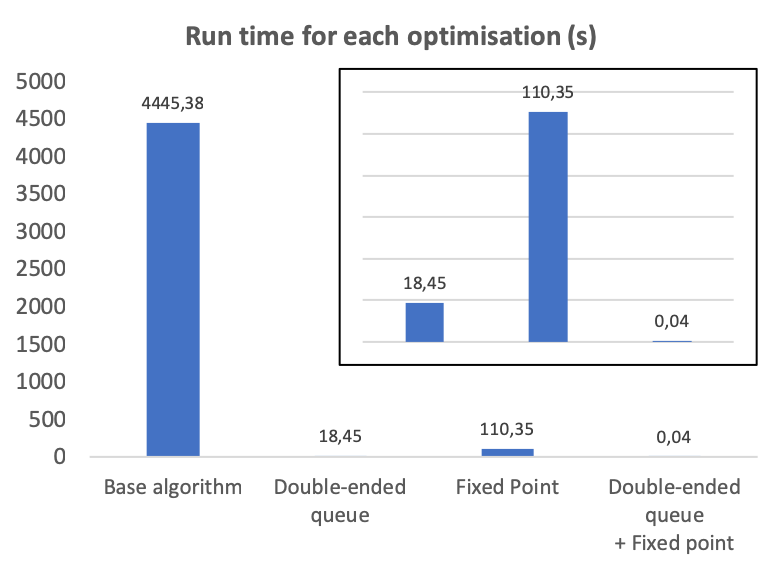
\includegraphics[height=4.8cm]{img/run_time}
  \quad 
  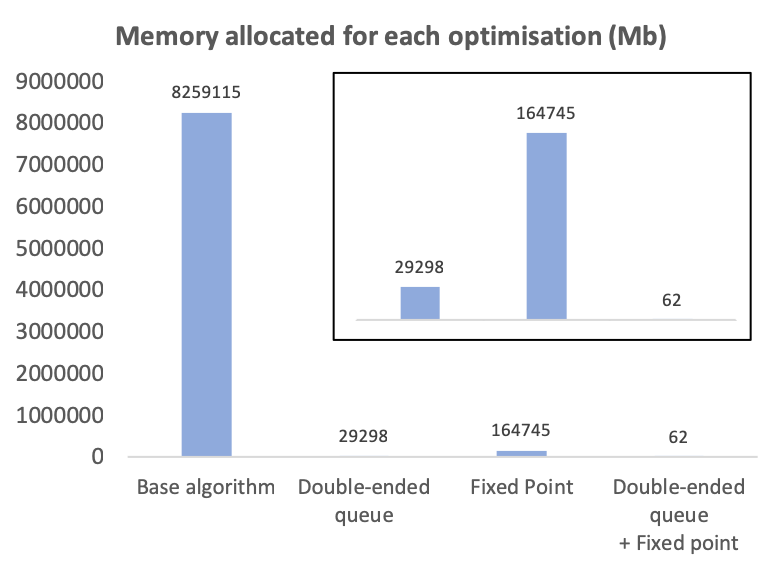
\includegraphics[height=4.8cm]{img/memory_alloc}	
  \caption{Running times (on the left) and memory allocated (on the
    right) when checking the bisimilarity of context-free session
    types on a test suite of 150 tests}
  \label{fig:results}
\end{figure}

When compared to the base algorithm, the running times and memory
allocated exhibit an improvement of more than 12,000,000\%. The
running time of the example in~\eqref{ex:chaotic} was brought down to
0.008 seconds.

% For this reasons, our proposal for an algorithm to
% check the equivalence of context-free session types stands on adapting
% the simplification stage to enable double-ended enqueueing and the
% computation of a fixed point at the simplification phase
% Listing~\ref{lst:enhanced} presents an enhanced version of the
% simplification stage coping the new proposals.

%%% Local Variables:
%%% mode: latex
%%% TeX-master: "main"
%%% End:
